\section{Half-Edge-Mesh}
Um die oben genannten Problemstellungen zu l\"osen, gibt es andere Ans\"atze Polygonalnetze zu realisieren. Einer dieser L\"osungen ist das Konzept der Half-Edge-Meshes. Ein solches Mesh besteht aus folgenden Komponenten: 
\begin{itemize}
	\item eine Liste von Vertices
	\item eine Liste von Half-Edges
	\item eine Liste von Faces.
\end{itemize}
Der Ansatz des Half-Edge-Mesh sieht dabei vor, dass jede Kante des Netzes aus zwei Half-Edges besteht, sodass jeweils eine Half-Edge auf einen Vertex der Kante zeigt, wie in Abbildung \ref{fig:half-edge-mesh} gezeigt.
Jede Half-Edge besitzt eine Referenz auf die ihr gegen\"uberliegende Half-Edge und auf die ihr Nachfolgende. Zudem referenziert sie die anliegende Face und den Vertex, aus dem sie hervorgeht.
\begin{figure}[t]
	\centering
	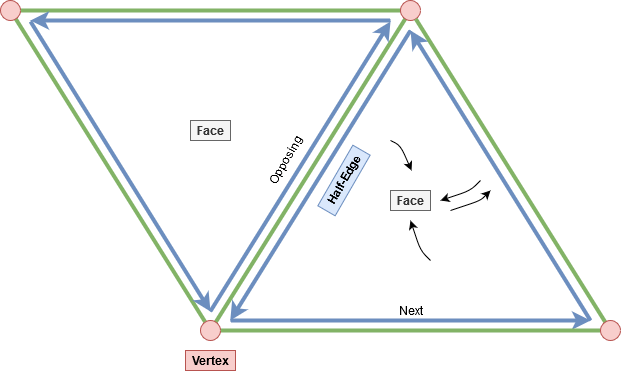
\includegraphics[width=0.7\linewidth]{Images/half-edge-mesh}
	\caption[Half-Edge-Mesh Schematik]{Die Elemente eines Half-Edge-Mesh.}
	\label{fig:half-edge-mesh}
\end{figure}

\subsection{Klassenstruktur}
Aus den beschriebenen Elementen einer Half-Edge-Netzstruktur ergibt sich das in Abbildung \ref{fig:classdiagramhalfedgemesh} gezeigte Klassendiagramm. Der grundlegende Aufbau der einzelnen Klassen basiert dabei auf dem Plankton-Mesh \cite{Meshmash2017}. Jede Komponente besitzt eine eigene Listenklasse. Allerdings besitzen die einzelnen Komponenten im Plankton-Mesh keine direkte Referenz auf die benachbarten Komponenten, sondern einen Verweis auf den Index der Elemente in der jeweiligen Liste. So hat eine Half-Edge keine weitere Half-Edge als ,,Next'', sondern ein den jeweiligen Index der n\"achsten Kante.

\subsection{Die Vertex, HalfEdge und Face Klassen}
Die Klassen \textit{Vertex, HalfEdge} und \textit{Face} sind die Datenmodelle der oben beschriebenen Komponenten. Die Vertex-Klasse besitzt einen \textit{Vector3} Point, der die Position im Raum darstellt, eine \textit{HalfEdge}, die von diesem Punkt aus geht (Im Gegensatz zu \cite{Meshmash2017} wird hier eine Referenz gespeichert.) und der Index des Punktes, um die Arbeit mit dem Unity-Mesh zu erleichtern. Zudem kann ein \textit{PositionChangedEvent} abonniert werden, um Positions\"anderungen im Unity-Mesh direkt zu zeigen.
\\
Eine Half-Edge besitzt die oben erw\"ahnten Eingenschaften: den Punkt von dem sie ausgeht, die anliegende Face, die gegen\"uberliegende und n\"achste HalfEdge sowie den Index der HalfEdge. Wie auch der Index der Vertices, ist dieser Index f\"ur das Unity-Mesh wichtig.
\\
Die Face-Klasse besitzt eine Referenz auf eine anliegende HalfEdge und den Index der Face, diese wieder f\"ur die Arbeit mit dem Unity-Mesh.

\subsection{Listenklassen}
Objekte der Klassen \textit{Vertex, HalfEdge, Face} werden jeweils in einer Listenklasse gespeichert. Die Klassen \textit{VertexList, HalfEdgeList, FaceList} implementieren das \textit{IEnumerable}-Interface, um die Iteration \"uber die Elemente zu vereinfachen. Zudem beinhalten diese Klassen die Kernlogiken f\"ur die Komponenten. VertexList bietet die M\"oglichkeit, einen neuen Vertex hinzuzuf\"ugen oder einen zu entfernen, die HalfEdgeList verf\"ugt \"uber eine  \textit{CreateHalfEdge}-Methode, die wie folgt eine HalfEdge anlegt:

\begin{lstlisting}

public HalfEdge CreateHalfEdge(Vertex vertex, Face face, HalfEdge next)
{
	var halfEdge = new HalfEdge(vertex, face, next, Count);
	vertex.HalfEdge = halfEdge;
	_halfEdges.Add(halfEdge);
	return halfEdge;
}

\end{lstlisting}

Und auch die FaceList besitzt eine Create-Methode, um eine Fl\"ache korrekt anlegen zu k\"onnen. Dabei wird die Referenz der Face auf die HalfEdge gesetzt und umgekehrt. Eine Weitere wichtige Methode ist die \textit{GetFaceCirculator}-Methode, die eine Liste aller HalfEdges, die an einer gegebenen Face anliegen, zur\"uck gibt.

\begin{figure}[t]
	\centering
	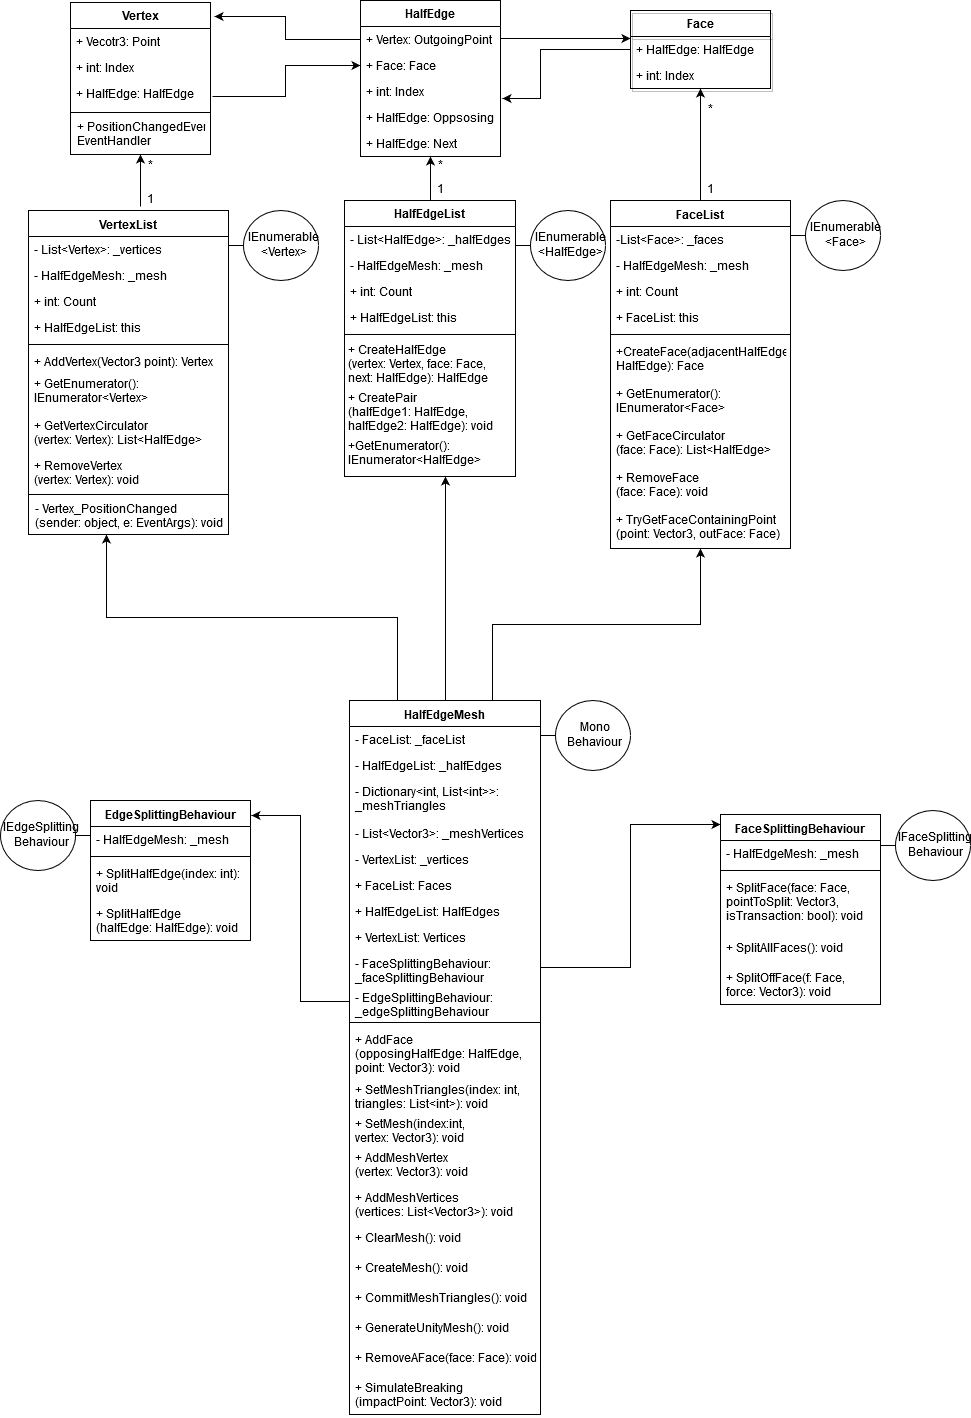
\includegraphics[width=0.7\linewidth]{Images/ClassDiagramHalfEdgeMesh}
	\caption[HalfEdgeMeshUMLDiagramm]{UML-Klassendiagramm des Half-Edge-Mesh Projekts}
	\label{fig:classdiagramhalfedgemesh}
\end{figure}


\section{Implementierung des Half-Edge-Meshes}
Die Oben genannten Listenklassen werden von der \textit{HalfEdgeMesh}-Klasse verwendet, um aus der beschriebenen Half-Edge-Datenstruktur ein von Unity renderbares Mesh zu erstellen. 
\\
Um ein Dreieck, die einfachste m\"ogliche Netzstruktur zu erzeugen, kann die Methode \textit{CreateMesh} verwendet werden. Diese erstellt die drei Eckpunkte des Dreiecks, verbindet zwei mit einer neuen Half-Edge und erzeugt damit ein Face. Die Fl\"ache wird dann verwendet um die fehlenden Kanten mit Referenzen zu erzeugen und anschlie{\ss}end wird die Referenz der ersten Half-Edge auf die zweite gesetzt. Zum Schluss wird \textit{GenerateUnityMesh} aufgerufen um mit den angelegten Daten das UnityMesh zu generieren.
\begin{lstlisting}

public void CreateMesh(Vector3 va, Vector3 vb, Vector3 vc)
{
	var a = Vertices.CreateVertex(va);
	var b = Vertices.CreateVertex(vb);
	var c = Vertices.CreateVertex(vc);

	var heA = HalfEdges.CreateHalfEdge(a, null, null);
	var face = Faces.CreateFace(heA);
	var heB = HalfEdges.CreateHalfEdge(b, face, heA);
	var heC = HalfEdges.CreateHalfEdge(c, face, heB);
	heA.Next = heC;

	GenerateUnityMesh();
}

\end{lstlisting}
Sollen beim erstellen des Netzes weitere Fl\"achen hinzugef\"ugt werden, ist es m\"oglich diese Methode zu erweitern oder weitere Faces mit \textit{AddFace} hinzuzuf\"ugen.

\subsection{GenerateUnityMesh}
Um aus den Daten des Half-Edge-Mesh ein f\"ur Unity brauchbares Mesh zu generieren, m\"ussen folgende Daten aus dem Half-Edge-Mesh entnommen werden: Die Position jedes Punktes, als Liste und ein Array mit der Reihenfolge, wie diese Punkte zu verbinden sind. Die Zusammenstellung dieser Daten passiert mit Hilfe von Linq. Hier der wichtigste Teil der \textit{GenerateUnityMesh}-Methode.
\begin{lstlisting}
	ClearMesh();
	// --- Add vertices
	var vertices = Vertices.Select(p => p.Point).ToList();

	// --- Add triangles
	foreach (var face in Faces)
	{
		var adjacentHalfEdges = Faces.GetFaceCirculator(face).ToList();
		SetMeshTriangles(face.Index, adjacentHalfEdges
		.Select(p => p.OutgoingPoint.Index).ToList(), true);
	}

	AddMeshVertices(vertices);
	CommitMeshTriangles();
\end{lstlisting}
Da das Netz eines komplexen Modells sehr gro{\ss} werden kann, ist es f\"ur die Laufzeit von Vorteil, wenn bei lokalen \"Anderungen nicht das gesamte Netz neu generiert werden muss, wobei jedes Mal \"uber alle Punkte, Kanten und Fl\"achen iteriert werden muss. Stattdessen werden alle Punkte zus\"atzlich in einer Liste gespeichert, die beim bearbeiten des Netzes das UnityMesh aktualisiert. Werden dem Half-Edge-Mesh neue Punkte hinzugef\"ugt, k\"onnen diese mit den Methoden \textit{AddMeshVertex} und \textit{AddMeshVertices} erg\"anzt werden. Am Ende der Methode wird die aktualisierte Liste dem UnityMesh \"ubergeben. 
\\
Auch die Triangles des UnityMeshes werden gecached. Da Manipulationen des Meshes in der Regel bedeuten, dass sich die Triangels relativ zu den drei Punkte einer Face ver\"andern, werden diese in dreier Tuplen in ein Dictionary geschrieben. Der Schl\"ussel ist dabei der Index der Face. Die Indexliste l\"asst sich mit \textit{SetMeshTriangles} bearbeiten. Dabei wird ein Eintrag an der Stelle des Faceindex hinzugef\"ugt, sofern er nicht vorhanden ist oder ver\"andert, falls ein Eintrag existiert. Wichtig ist dies zum Beispiel, wenn eine Face geteilt wird und ein Dreieckseintrag mit zwei von drei Punkten \"ubernommen wird. Als weiteren Parameter kann angegeben werden, ob eine Ver\"anderung Teil einer gr\"o{\ss}eren Transaktion war, um zu vermeiden, dass bei umfangreicheren Operationen, wie der Subdivision aller Faces, f\"ur jeden Methodenaufruf das Dictionary in eine Liste umzuwandeln und das Mesh erneut rendern zu m\"ussen. Wird diese Option verwendet, muss nach Abschluss der Transaktion \textit{CommitMeshTriangles} ausgef\"uhrt werden, um die \"Anderungen ins Mesh zu \"ubernehmen.